\documentclass[conference]{IEEEtran}
\IEEEoverridecommandlockouts
% The preceding line is only needed to identify funding in the first footnote. If that is unneeded, please comment it out.
\usepackage{cite}
\usepackage{amsmath,amssymb,amsfonts}
\usepackage{algorithmic}
\usepackage{graphicx}
\usepackage{textcomp}
\usepackage{xcolor}
\usepackage{hyperref}
\usepackage{mytodonotes}
\usepackage{cleveref}
\def\BibTeX{{\rm B\kern-.05em{\sc i\kern-.025em b}\kern-.08em
    T\kern-.1667em\lower.7ex\hbox{E}\kern-.125emX}}
\begin{document}

\title{HarmoniKt: a Unifying Middleware for Heterogeneous Robot Swarms}


\author{
\IEEEauthorblockN{Manuel Andruccioli}
\IEEEauthorblockA{%\textit{dept. name of organization (of Aff.)} \\
\textit{University of Bologna}\\
Cesena, Italy \\
manuel.andruccioli@unibo.it}
\and
\IEEEauthorblockN{Angela Cortecchia}
\IEEEauthorblockA{%\textit{dept. name of organization (of Aff.)} \\
\textit{University of Bologna}\\
Cesena, Italy \\
angela.cortecchia@unibo.it}
\and
\IEEEauthorblockN{Davide Domini}
\IEEEauthorblockA{%\textit{dept. name of organization (of Aff.)} \\
\textit{University of Bologna}\\
Cesena, Italy \\
davide.domini@unibo.it}
\and
\IEEEauthorblockN{Nicolas Farabegoli}
\IEEEauthorblockA{%\textit{dept. name of organization (of Aff.)} \\
\textit{University of Bologna}\\
Cesena, Italy \\
nicolas.farabegoli@unibo.it}
\and
\IEEEauthorblockN{Silvia Mirri}
\IEEEauthorblockA{%\textit{dept. name of organization (of Aff.)} \\
\textit{University of Bologna}\\
Cesena, Italy \\
silvia.mirri@unibo.it}
\and
\IEEEauthorblockN{Danilo Pianini}
\IEEEauthorblockA{%\textit{dept. name of organization (of Aff.)} \\
\textit{University of Bologna}\\
Cesena, Italy \\
danilo.pianini@unibo.it}
\and
\IEEEauthorblockN{Riccardo Venanzi}
\IEEEauthorblockA{%\textit{dept. name of organization (of Aff.)} \\
\textit{University of Bologna}\\
Bologna, Italy \\
riccardo.venanzi@unibo.it}
\and
\IEEEauthorblockN{Mirko Viroli}
\IEEEauthorblockA{%\textit{dept. name of organization (of Aff.)} \\
\textit{University of Bologna}\\
Cesena, Italy \\
mirko.viroli@unibo.it}
}

% \author{
% \IEEEauthorblockN{
% Manuel Andruccioli,
% Angela Cortecchia,
% Davide Domini,
% Nicolas Farabegoli,\\
% Silvia Mirri,
% Riccardo Venanzi,
% Mirko Viroli
% }
% \IEEEauthorblockA{
% \textit{University of Bologna}\\
% Cesena, Italy \\
% \{manuel.andruccioli, angela.cortecchia, davide.domini, nicolas.farabegoli,\\
% silvia.mirri, riccardo.venanzi, mirko.viroli\}@unibo.it
% }
% }

\newcommand{\approach}{\textsc{HarmoniKt}}

\maketitle

\begin{abstract}
In recent years, 
 companies have increasingly invested in Industry 4.0 research 
 to automate repetitive tasks or activities that may be harmful to humans. 
% 
For instance, 
 large-scale warehouses such as those operated by Amazon rely heavily 
 on mobile robots to streamline logistics operations and ensure worker safety. 
% 
At the same time, 
 robot manufacturers are releasing more reliable platforms with advanced capabilities, 
 making them suitable for complex industrial tasks. 
% 
Despite this growing interest and technological progress, 
 significant challenges remain. 
% 
A key and non-trivial issue lies in the integration of heterogeneous robot fleets: 
 each vendor typically employs proprietary technologies and interfaces, 
 which hinders interoperability and limits the potential of multi-brand deployments.

In this work, 
 we introduce \approach{}, 
 an extensible middleware that addresses this challenge by introducing an abstraction layer 
 and providing a unified REST API for the control and management of heterogeneous robots. 
% 
Our solution has been validated in a physical industrial-like environment using a mixed fleet 
 of Boston Dynamics Spot and Mobile Industrial Robots (MiR). 
%
Furthermore, we present a comparative analysis showing that the access latency introduced 
 by our middleware is not significantly higher than that of direct robot access, 
 demonstrating the feasibility of unified robot management without compromising performance.
\end{abstract}

\begin{IEEEkeywords}
component, formatting, style, styling, insert
\end{IEEEkeywords}


\section{Introduction}\label{sec:intro}

\subsection{Context}
In the era of Industry 4.0, 
 the drive toward automation has intensified across manufacturing, 
 logistics, and service domains. 
% 
Many enterprises are investing heavily in research and deployment of robotic systems 
to take over repetitive tasks, reduce human exposure to hazardous environments, 
 and improve throughput and consistency. 
% 
Warehouse operations are a quintessential example: 
 major players like Amazon employ thousands of autonomous mobile robots to move inventory, 
 reduce picking times, and eliminate manual transport in large-scale facilities.
%
At the same time, the robotics industry has matured: 
 companies now produce platforms with increasing reliability, rich sensing suites, versatile locomotion, 
 and capability to execute complex behaviors (navigation, manipulation, perception). 
% 
The promise is that robotic fleets will become standard building blocks of the modern smart factory.

Yet, even with escalating investments and advancing robotics capabilities, 
 several challenges remain before these systems can fully deliver on their potential at scale.

\subsection{Research Gap}

One of the major nontrivial obstacles is integration of heterogeneous robot fleets. 
%
In practice, 
 each manufacturer typically employs its own software stack, proprietary APIs, 
 communication protocols, and control paradigms. 
% 
This heterogeneity makes combining robots from multiple vendors into a seamless, 
 interoperable fleet extremely difficult, which in turn constrains system designers 
 to single-vendor lock-in or expensive custom wrappers. 
% 
In the literature of robot fleet management, 
 authors often note that much work focuses on task allocation, path planning, scheduling, 
 but relatively less tackles the problem of unified access and control across diverse platforms. 

Some middleware proposals have attempted to address interoperability in both industrial and academic contexts. 
%
For instance,
 TalkRoBots~\cite{ayaida2022fi} introduces a unified communication approach that bridges ROS, proprietary robot frameworks, 
 and IIoT devices in Industry 4.0 environments. 
% 
Zegarra et al.~\cite{cuadroszegarra2024jsan}, instead, propose an Internet of Robotic Things (IoRT) approach 
 to unify communication among different robot operating systems, focusing primarily on network-level interoperability 
 rather than providing unified control APIs. 
% 
The Pluggable Distributed Resource Allocator (PDRA)~\cite{rossi2020iros} presents a middleware layer that enables robots 
 to share computational tasks by intercepting executor requests and routing them across the fleet 
 to optimize energy consumption and latency. 
% 
While effective in distributed resource management, 
PDRA primarily addresses compute-resource sharing rather than unified control of heterogeneous robotic hardware. 
%
Similarly, in mission coordination contexts, architectures such as MissionControl~\cite{rodrigues2022jss} 
 support coalition formation among diverse robots, yet they still leave open the challenge of offering 
 a standardized control API across vendor-specific stacks.
%
Moreover, the trade-off between abstraction overhead and performance (e.g., latency, throughput) 
 is seldom thoroughly evaluated in real-world heterogeneous fleets.

\subsection{Contribution}
In this work, 
 we address precisely this gap by presenting \approach{}:
 an extensible middleware for unifying access to heterogeneous robot fleets. 
% 
\approach{} introduces an abstraction layer over diverse robot APIs and control paradigms, 
 exposing a common REST API for commanders or higher-level applications to issue motion commands, 
 query status, and orchestrate task execution, regardless of robot make or model. 
% 
Our architecture is modular and pluggable, 
 allowing future extensions to additional robot types and communication protocols with minimal effort.

We validate \approach{} in a physical testbed combining Boston Dynamics Spot robots 
 and MiR (Mobile Industrial Robots) platforms in an industrial-style environment. 
% 
We report on implementation challenges, integration strategies, and runtime behavior. 
%
Importantly, we include a comparative performance study: 
 we measure access latency through \approach{} and compare it to direct native access to each robot, 
 showing that the overhead introduced by our abstraction is limited and acceptable for practical deployments. 
% 
Thus, we demonstrate that unified robot management is feasible without significant performance compromise.


Finally, 
 to foster reproducibility and community adoption, 
  \approach{} has been released as open-source software 
  on GitHub\footnote{\url{https://github.com/HarmoniKt/HarmoniKt}} 
  under a permissive license, enabling researchers and practitioners to freely use, extend, 
  and integrate the framework into their own applications.

\subsection{Outline}
The rest of the paper is organized as follows:
 \Cref{sec:related} provides background and related works;
 \Cref{sec:arc} introduces \approach{} disscussing both the high level architecture and the implementation;
 \Cref{sec:eval} provides details on the real world evaluation;
 \Cref{sec:impact} discusses possible impacts of \approach{};
 and \Cref{sec:future} concludes the paper and outlines future research directions.

\section{Background and Related Works}\label{sec:related}

\subsection{Case Study Platforms: Boston Dynamics Spot and MiR}

To validate our middleware, 
 we selected two complementary and representative robotic platforms (\Cref{fig:robots}), namely: 
 the Boston Dynamics Spot quadruped\footnote{\url{https://bostondynamics.com/products/spot/}}
 and the Mobile Industrial Robots (MiR) mobile base\footnote{\url{https://mobile-industrial-robots.com/}}.

\begin{figure}[htb]
    \centering
    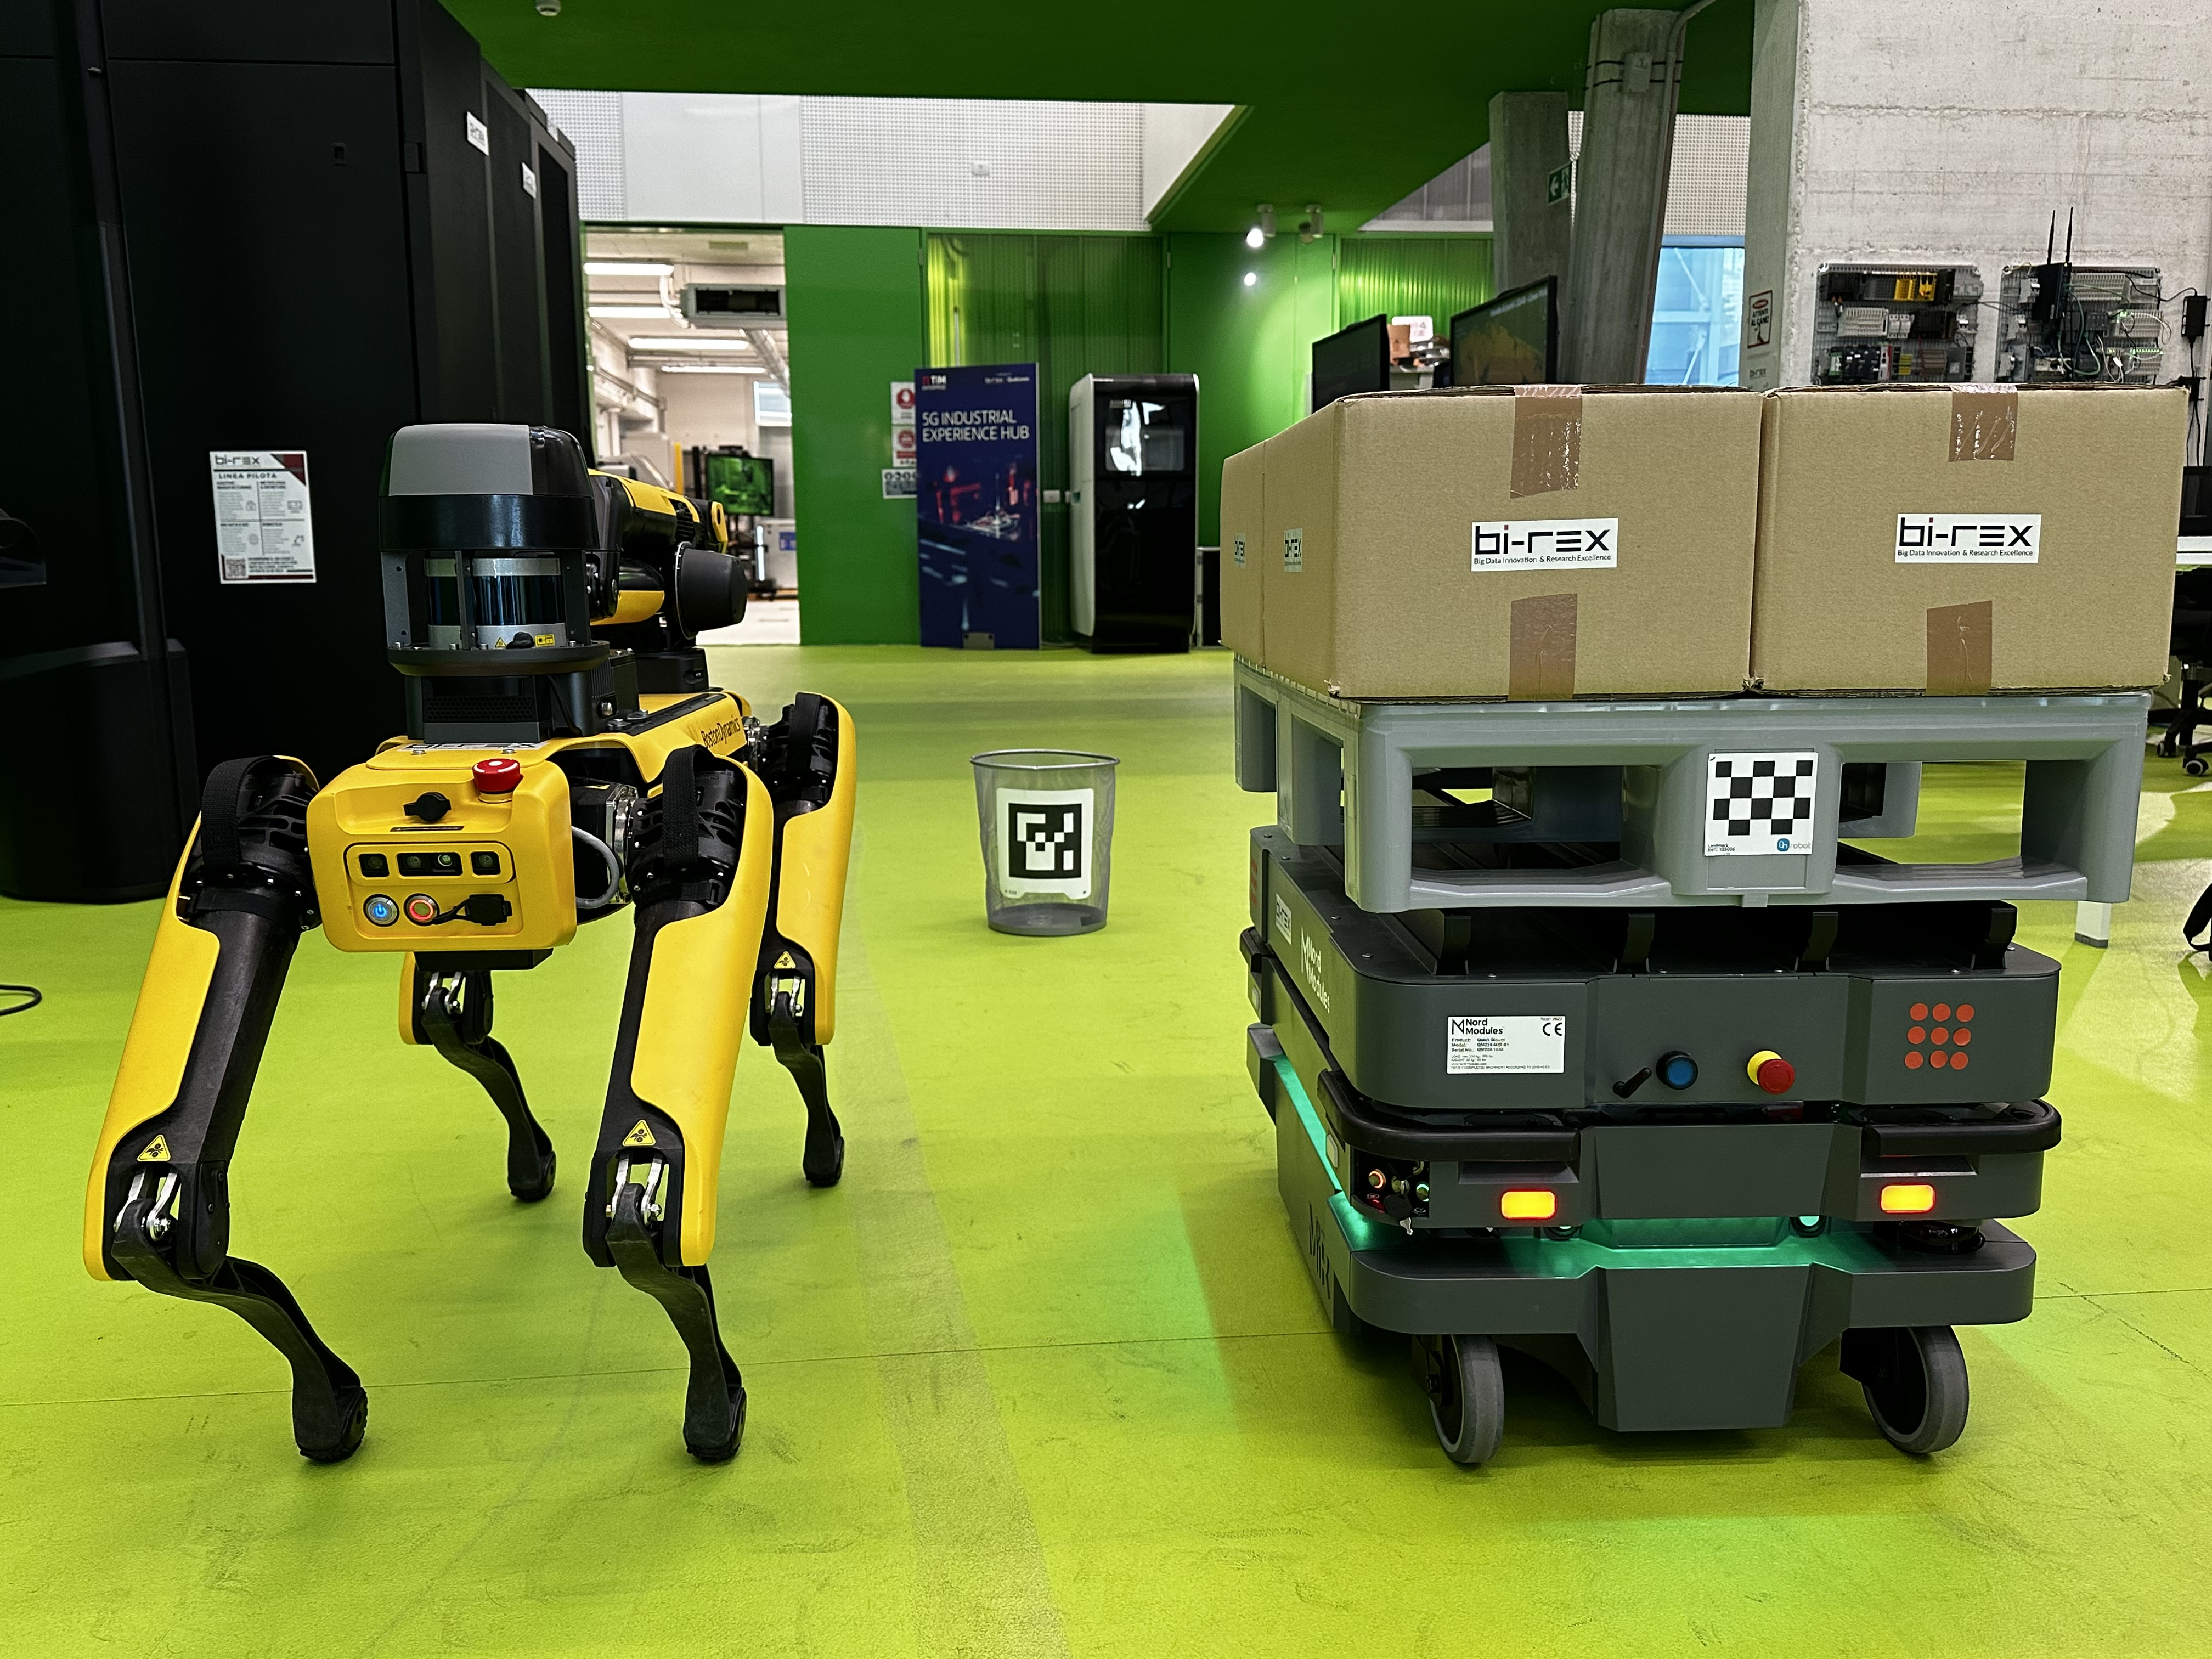
\includegraphics[width=1\columnwidth]{images/robots.jpeg}
    \caption{
        TBD.
    }
    \label{fig:robots}
\end{figure}

Spot is a versatile quadruped robot designed for unstructured and dynamic environments. 
%
Its legged locomotion allows it to traverse stairs, rough terrain, 
 and cluttered industrial facilities where wheeled platforms would struggle. 
% 
Equipped with a rich sensor suite including stereo cameras, IMUs, and optional LIDAR payloads, 
 Spot can perform inspection, mapping, and payload-carrying tasks. 
% 
Its SDK (primarily Python-based) enables programmatic access to locomotion primitives, perception data, 
 and autonomy modules, making it suitable for research and industrial deployment alike. 
% 
In Industry 4.0 scenarios, Spot is often used for safety inspections in hazardous areas, 
 surveying environments with thermal or gas sensors, 
 or assisting in monitoring tasks that are unsafe for humans.

In contrast, the MiR family of robots represents one of the most widely adopted 
 autonomous mobile robot (AMR) platforms in logistics and manufacturing.
%
MiR robots are wheeled, indoor-oriented AMRs specifically designed for material handling, warehouse logistics, 
 and line-feeding tasks in production facilities. 
% 
They provide reliable obstacle avoidance, map-based navigation, 
 and fleet management through proprietary software. 
% 
Unlike Spot, their strengths lie in efficiency, payload capacity, and integration 
 with industrial workflows such as transporting carts and pallets.

The combination of Spot and MiR provides a testbed with heterogeneous 
 locomotion modalities, APIs, and use cases: 
  a legged robot designed for unstructured inspection tasks, 
  and a wheeled robot specialized for structured intralogistics. 
%
This heterogeneity exemplifies the integration challenges faced in Industry 4.0, 
 where companies seek to combine different robot types into a cohesive fleet 
 to maximize operational flexibility.

\subsection{Microservices Architecture for IIoT Middlewares}
In recent years, 
 the microservices architectural style has become a dominant paradigm in modern software engineering 
  due to its ability to support modularity, scalability, and maintainability. 
%  
Organizations are increasingly moving away from monolithic applications toward collections of independent services, 
 each encapsulating a well-defined functionality.
 %
 A large-scale O'Reilly study of industry adoption reported that more than $60\%$ 
  of surveyed organizations had already deployed microservices in production, 
  and nearly one third were migrating most of their systems to this architectural 
  style\footnote{\url{https://www.oreilly.com/radar/microservices-adoption-in-2020/}}. 
%  
More recent empirical studies confirm that microservices are valued for enabling scalability, 
 independent deployment, and technological flexibility, although they introduce challenges related to 
 testing, monitoring, and data consistency~\cite{nogueira2024icsm}.

This trend is visible not only in robotics 
 but across the Internet of Things (IoT) and Industrial IoT (IIoT) domains. 
% 
For instance, a recent microservice-based middleware for IIoT~\cite{venanzi2021globecom} demonstrates how 
 sensor, device, and application modules can be composed as independent services interacting via RESTful APIs, 
  achieving elasticity and modular updates without disrupting the system as a whole. 
%  
Although not explicitly designed for robotic control, 
 this work illustrates the applicability and benefits of microservices in 
  industrial-scale, heterogeneous environments, and strengthens the case 
  for adopting a similar approach in robot middleware.

In the robotics domain, modular approaches have also emerged. 
%
Some recent works on mobile robots propose microservice-based control architectures 
 that decouple motion planning, perception, and safety modules into independent services, 
 coordinated through well-defined interfaces~\cite{DBLP:journals/ras/SchrickHTK25}. 
% 
Similarly, Xia et al.~\cite{DBLP:journals/ras/XiaZWCL18} propose a microservice-based cloud robotics architecture, 
 modularizing functionalities such as SLAM, navigation, and vision into containerized services,
 and validate their design via experiments on real robots in intelligent spaces.
% 
These examples highlight how the microservices approach can provide the flexibility required 
 to support interoperability and scalability in robotics and Industry 4.0 environments.

\subsection{Related Works}
The problem of integrating heterogeneous robot fleets has been addressed 
 by several academic and industrial initiatives, though with varying focus and maturity.

\paragraph{Early Robotics Middleware} 
Foundational frameworks such as Player/Stage~\cite{vaughan2003player} 
 and MIRO~\cite{DBLP:journals/trob/UtzSEK02} demonstrated the importance 
 of hardware abstraction and standardized communication. 
% 
In particular, Player offered a device server model where heterogeneous robots could be accessed via uniform interfaces, 
 while Stage provided multi-robot simulation capabilities. 
% 
These frameworks established the principles of separating robot hardware details from higher-level applications, 
 though their focus was largely on academic and simulation contexts.

\paragraph{ROS and Component-Based Platforms} 
The Robot Operating System (ROS)~\cite{quigley2009ros} has become the de facto standard in academia, 
 providing a publish/subscribe architecture and modular drivers. 
% 
While ROS facilitates code reuse and integration, it was not originally designed for large heterogeneous fleets, 
 and multi-robot deployments often require complex configurations. 
% 
Other component-oriented middleware such as RT-Middleware~\cite{DBLP:conf/iros/AndoSKKY05} 
 and OPRoS~\cite{jang2010opros} introduced standardized service/component models 
 to promote interoperability, though adoption has been limited.

\paragraph{Fleet Management Systems} 
Recent work has turned toward full fleet management solutions. 
%
The Open-RMF framework\footnote{\url{https://www.open-rmf.org/}} is an open-source platform 
 enabling interoperability among different mobile robot fleets and shared infrastructure (e.g., elevators, doors). 
% 
Field deployments, such as at Tartu University Hospital, have demonstrated its ability 
 to manage heterogeneous AMRs in real-world settings. 
% 
Industry standards like VDA 5050~\cite{franke2023identification} 
 and OPC UA Robotics Companion Specification~\cite{DBLP:conf/etfa/ProfanterB0K19} 
 aim to unify communication between fleet management systems and robots, 
 particularly in logistics and manufacturing domains. 
%  
These initiatives illustrate the industrial push toward vendor-agnostic fleet orchestration.

\paragraph{Recent Middleware Proposals} 
In academic contexts, Ayaida et al. introduced TalkRoBots~\cite{ayaida2022fi}, 
 a middleware bridging ROS and proprietary systems to enable communication 
 across heterogeneous robots in Industry 4.0 scenarios. 
% 
Similarly, Zegarra et al.~\cite{cuadroszegarra2024jsan} proposed an IoRT-based middleware 
 to unify communication at the network level among different robot operating systems. 
% 
On the other hand, resource allocation approaches such as PDRA~\cite{DBLP:conf/iros/RossiVNSH20} 
 focus on distributed compute sharing among robots, 
 while architectures like MissionControl~\cite{DBLP:journals/jss/RodriguesCAMRP22} 
  target multi-robot coalition formation and mission assignment. 
%  
These works contribute to interoperability or coordination but often lack the comprehensive abstraction 
 and unified API layer required for seamless fleet integration.

\subsection{Motivation}
The survey of existing frameworks shows that, 
 despite significant progress in robotics middleware and fleet management, important limitations remain. 
% 
Many approaches are constrained by vendor-specific technologies, limited scalability, 
 or proof-of-concept maturity, and only a few are validated in real industrial environments. 
% 
Moreover, the trade-off between abstraction and performance is often underexplored, 
 leaving open questions about the feasibility of unified control at scale. 
% 
These gaps motivate our contribution: 
 \approach{} addresses interoperability challenges by combining a microservices-based architecture 
  with unified REST APIs, thereby bridging the flexibility of academic proposals 
   bwith the robustness and standardization efforts emerging from industry.

\section{\approach{} Middleware}\label{sec:arc}
\subsection{Architecture}

\begin{figure}[htb]
    \centering
    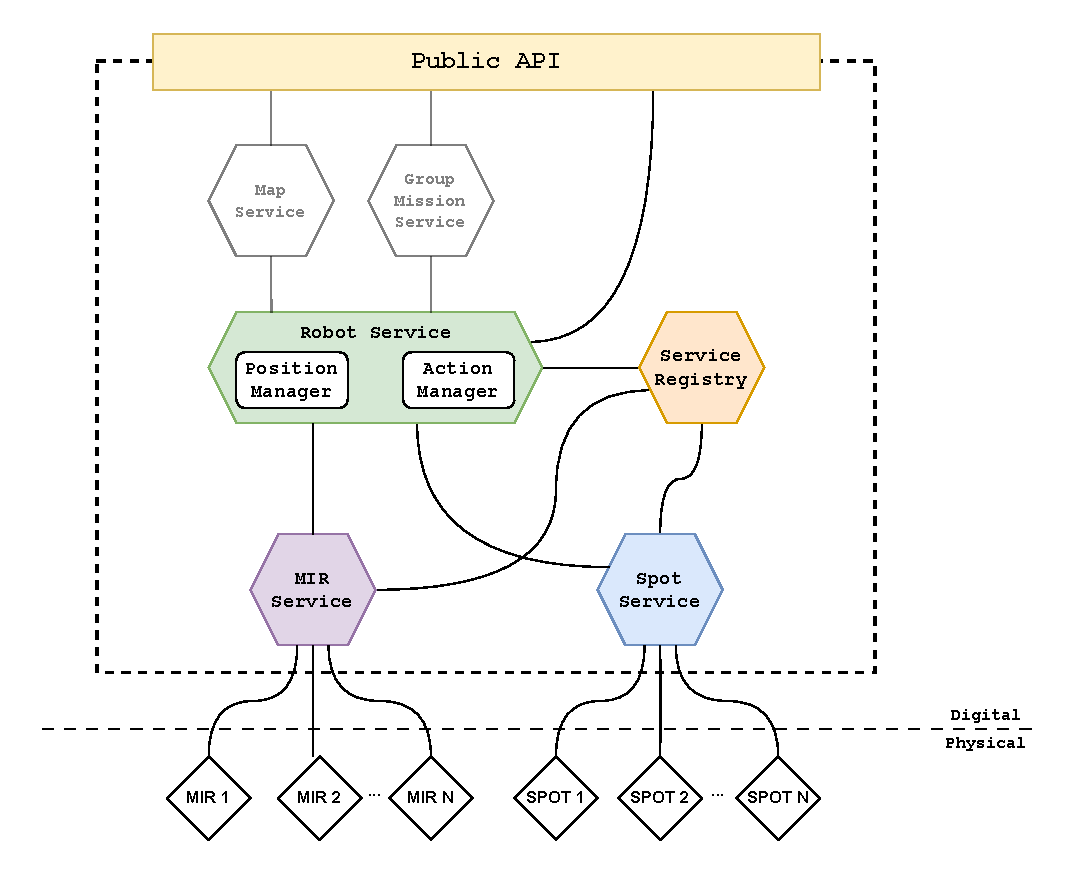
\includegraphics[width=1\columnwidth]{images/arc.pdf}
    \caption{
        TBD.
    }
    \label{fig:arc}
\end{figure}

\approach{} is designed around a distributed microservices architecture, 
 following the principle of clear separation of concerns. 
% 
Each service encapsulates a well-defined responsibility, 
 enabling independent deployment, failure isolation, and flexible scalability. 
% 
This design allows the middleware to accommodate heterogeneous robot platforms 
 without requiring modifications to the overall system.

At the core lies the \texttt{robot-service}, 
 which functions as the orchestration hub. 
% 
It exposes a unified REST API to client applications 
 and abstracts away the complexity of vendor-specific interfaces. 
% 
Robot-specific functionality is delegated to dedicated services: 
 the \texttt{spot-service}, implemented in Python to leverage Boston Dynamics' official SDK, 
 and the \texttt{mir-service}, developed in Kotlin to handle the Mobile Industrial Robots platform. 
% 
This polyglot design is a central feature of \approach{}: 
 by allowing each service to be implemented in the language 
 and ecosystem best suited to the corresponding robot or functionality,
  the middleware can fully exploit vendor-provided SDKs and libraries 
  while still exposing a uniform interface to external consumers. 
%  
This flexibility is not incidental but rather essential to achieving our objectives of 
 extensibility, interoperability, and maintainability across heterogeneous robotic platforms.

Additional services are also foreseen to provide shared functionality across the fleet. 
%
In particular, a \texttt{map-service} is planned to manage spatial data and navigation maps, 
 enabling robots to access common localization and environment representations, 
 while a \texttt{group-mission-service} is envisioned to coordinate multi-robot tasks, 
 allowing heterogeneous agents to participate in collaborative missions. 
% 
Although these services have not yet been implemented, 
 their design has been integrated into the overall architecture, 
 ensuring that the system can be readily extended in future developments.

This modular architecture makes \approach{} inherently extensible: 
 integrating a new robot type requires deploying a new service that conforms to the established interface contracts, 
 without modifying the rest of the platform. 
% 
The design therefore combines abstraction, extensibility, and interoperability, 
 aligning with the requirements of Industry 4.0 environments where diverse robotic assets 
 must be orchestrated under a unified framework.

\subsection{Implementation}
The middleware is implemented using a polyglot technology stack carefully selected to 
 balance reliability, developer productivity, and integration with vendor tools. 
% 
The majority of services are developed in Kotlin using the Ktor framework, 
 chosen for its concise syntax, type safety, and seamless integration with the JVM ecosystem. 
% 
The Spot integration service, however, is written in Python, reflecting the availability 
 and maturity of Boston Dynamics' official SDK. 
% 
All inter-service communication is HTTP-based, ensuring language-agnostic interoperability.

The system relies on several infrastructure components to achieve robustness and maintainability. 
%
Consul provides service discovery and health checks, 
 enabling automatic registration and dynamic routing among services. 
% 
Docker and Docker Compose are used for containerization and orchestration, 
 ensuring consistent deployments across environments and simplifying scaling. 
% 
A Caddy server acts as a reverse proxy and API gateway, 
 handling request routing, TLS termination, and centralized access control. 
% 
Build and deployment pipelines are automated via Gradle with Kotlin DSL, GitHub Actions for CI/CD, 
 and Renovate for dependency management, ensuring that the codebase remains secure and up to date.


\section{Evaluation}\label{sec:eval}
\clearpage

\section{Opportunities and Challenges}\label{sec:impact}

While \approach{} already demonstrates the feasibility of unifying 
 heterogeneous robots under a common abstraction, 
 several challenges and opportunities emerge from its current design and envisioned extensions.

A central challenge lies in the realization of the \texttt{map-service}, 
 which is intended to provide a unified spatial representation accessible to all robots in the fleet. 
% 
Designing such a service requires careful engineering to integrate diverse mapping formats 
 and localization methods across vendors, while ensuring consistency, scalability, and extensibility. 
% 
Achieving this goal would enable seamless coordination among heterogeneous agents 
 but entails significant complexity in data fusion and synchronization.

In contrast, 
 the planned \texttt{group-mission-service} opens a wide avenue for future developments. 
% 
By exposing a unified API for multi-robot coordination, 
 this service could enable high-level orchestration at the swarm level. 
% 
The field of swarm robotics~\cite{brambilla2013swarm} has grown rapidly in recent years, 
 fueled both by advances in artificial intelligence and by novel programming paradigms. 
% 
On the AI side, 
 breakthroughs in multi-agent reinforcement learning (MARL)~\cite{DBLP:journals/tsmc/BusoniuBS08,malucelli2025sac} 
 allow robot collectives to acquire complex cooperative behaviors 
 through trial-and-error interactions with the environment. 
% 
Preliminary studies have also compared learning-based methods with more traditional control approaches 
 such as PID controllers for autonomous vehicle coordination~\cite{DBLP:conf/smartcomp/BravettiBTAOG25}, 
 raising the need for real-world validation beyond simulation. 
% 
\approach{}, by providing unified access to diverse physical robots, 
 offers a unique testbed where such comparisons can be performed under realistic conditions.

Beyond learning-based approaches, 
 recent research has also explored macroprogramming paradigms, 
 notably aggregate computing (AC)~\cite{beal2015computer,cortecchia2024acsossymp}, 
 which shift the programming abstraction from individual robots to the collective. 
% 
These paradigms have already proven effective in developing coordination logic for large-scale IoT 
 and complex systems~\cite{cortecchia2024acsos},
 showing strong potential for swarm robotics~\cite{aguzzi2025lmcs,DBLP:conf/coordination/AguzziBBCCDFPV25}. 
% 
Moreover, they can be naturally integrated with AI-based techniques, 
 combining the scalability of collective abstractions with the adaptiveness 
 of machine learning~\cite{domini2024scp}. 
% 
\approach{} could play a pivotal role as an enabling platform for experimenting with these hybrid approaches.

Another promising direction stems from the broader edge-cloud continuum. 
%
In modern industrial environments, 
 computational resources are distributed across centralized servers and edge devices. 
% 
This opens the opportunity for dynamic task allocation strategies that optimize 
 energy consumption, robot battery life, or latency 
 of mission-critical tasks~\cite{domini2024woa}. 
% 
While much of the existing research in this space has been validated primarily in simulation, 
 \approach{} provides a concrete environment to test such strategies in the field, 
 thereby advancing their maturity.

Finally, emerging efforts in human-robot interaction point to the use of large language models (LLMs) 
 as natural interfaces for commanding robot fleets~\cite{olaiya2025natural,aguzzi2025language}. 
% 
By leveraging natural language, operators could issue high-level instructions without requiring 
 detailed programming or vendor-specific knowledge. 
% 
Since \approach{} already abstracts vendor APIs into a unified interface, 
 it could serve as the foundation for integrating LLM-based frontends, 
 effectively bridging human operators and heterogeneous fleets in an intuitive and scalable manner.

In summary, \approach{} not only addresses current interoperability challenges 
 but also paves the way for novel research directions at the intersection of 
 swarm robotics, artificial intelligence, distributed systems, and human-robot interaction. 
% 
While technical hurdles such as unified mapping remain, 
 the platform's extensibility and real-world grounding create unique opportunities 
 for advancing both academic research and industrial practice.


\section{Conclusions and future work}\label{sec:future}

\section*{Acknowledgment}
We would like to thank the BI-REX Competence Center for providing access to their robot fleet and 
 laboratory facilities, which enabled us to test the middleware in a real-world environment closely 
  resembling that of a modern Industry 4.0 setting.


\bibliographystyle{IEEEtran}
\bibliography{IEEEexample}

\end{document}
